\chapter{Externe Algorithmen}

\begin{minipage}{.6\textwidth}
  Greift man auf sehr große Datenbestände zu, so sind diese in der Regel auf Sekundärspeicher wie Platte oder Band gespeichert, weil diese sehr günstig sind. Problem ist, dass der Zugriff auf den Speicher sehr viel Zeit benötigt.
  
  \term{Externe Algorithmen}\index{Externe Algorithmen} nehmen an, dass die \emph{interne Arbeit}, also die Rechenarbeit, kostenlos ist. Minimiert werden soll die Anzahl an Zugriffen auf den Sekundärspeicher.
\end{minipage}
\hfill
\begin{minipage}{.35\textwidth}
  \begin{figure}[H]
    \includegraphics[width=\textwidth]{externalModel}
    \caption{Sekund"ärspeicher-Modell mit schnellem internen Speicher der Größe \( M \) und einem beliebig großem externen Speicher, der über einen \( B \) Wörter breiten Bus angebunden ist}
  \end{figure}
\end{minipage}

\section{Externe Stapel}
Wir haben 2 interne Puffer mit Speicherplatz von je $B$ Wörtern. Für das Lesen und Schreiben ist amortisiert jeweils eine Laufzeit von $O(1/B)$ nötig, da bei Über-/Unterlauf jeweils ein Puffer als Block auf den/vom externen Speicher geschrieben/gelesen wird.

\section{Externes Sortieren}

\section{Mehrwegemischen, externes Mischen}

Als nichttriviales Beispiel werden wir \term{Mehrwegemischen}\index{Mehrwegemischen} betrachten:

\begin{pseudocode}
  \textbf{\textsc{multiwayMerge}}\( (a_1,\dots,a_k,c : \text{File \textbf{of} Element}) \) \\
  \phantom{\enskip} \textbf{for} \( i \coloneqq 1 \) \textbf{to} \( k \) \textbf{do} \( x_i \coloneqq a_i\text{.readElement} \) \\
  \phantom{\enskip} \textbf{for} \( j \coloneqq 1 \) \textbf{to} \( \sum_{i=1}^k \left\vert a_i \right\vert \) \textbf{do} \\
  \phantom{\enskip} \phantom{\enskip} find \( i \in 1\dots k \) that minimizes \( x_i \) \enskip{} \textcolor{gray}{// no IOs, \( O(\log k) \) time} \\
  \phantom{\enskip} \phantom{\enskip} \( c\text{.writeElement}(x_i) \) \\
  \phantom{\enskip} \phantom{\enskip} \( x_i \coloneqq a_i\text{.readElement} \)
\end{pseudocode}

Der Aufwand beträgt

\begin{itemize}
  \item \textbf{I/O}: \( a_i \) lesen \( \approx \frac{\left\vert a_i \right\vert}{B} \), \( c \) schreiben \( \approx \sum_{i=1}^k \frac{\left\vert a_i \right\vert}{B} \)

  \( \Rightarrow \) Insgesamt \( \leq \approx 2\frac{\sum_{i=1}^k \left\vert a_i \right\vert}{B} \)

  \emph{Bedigungung}: wir brauchen \( k+1 \) Pufferblöcke.
\end{itemize}

\subsection{Sortieren durch Mehrwegemischen mittels Run Formation}
Ähnlich zu Merge Sort. Sortiere jeweils Eingabeportionen in sogenannten Runs der Größe $M$. Zunächst wurde das binäre Mischen mit $M/N = 2$ betrachtet. Mehrwegemischen ist eine Generalisierung dessen, welche eine bessere Laufzeit durch verringerung der Mischphasen erzielt.
 
Wir können dann Mehrwegemischen verwenden, um zu sortieren: 

\begin{enumerate}
  \item Sortiere \( \left\lceil \tfrac{n}{M} \right\rceil \) Runs mit je \( M \) Elementen.
  \item Mische jeweils \( \tfrac{M}{B} \) Runs, bis nur noch ein Run übrig ist.
\end{enumerate}


Die Anzahl an I/Os setzt sich aus \( 2\tfrac{n}{B} \) I/Os für das Sortieren, \( 2\tfrac{n}{B} \) I/Os für das Mischen und \( \left\lceil \log_{M/B} \tfrac{n}{M} \right\rceil \) Mischphasen zusammen, insgesamt also

\begin{equation*} 
  \text{sort}(n) \cong \frac{2n}{B}\left( 1 + \left\lceil \log_{M/B} \frac{n}{M} \right\rceil \right) \enskip \text{I/Os.}
\end{equation*}

Die interne Arbeit setzt sich aus
\begin{itemize}
  \item Run formation: \( O(n\log M) \),
  \item Zugriffe auf die Prioritätsliste pro Phase: \( O\left( n\log \tfrac{M}{B} \right) \),
  \item Anzahl Phasen: \( \left\lceil \log_{M/B} \tfrac{n}{M} \right\rceil \)
\end{itemize}
zusammen, insgesamt ergibts dich die Laufzeit dann zu:

\begin{equation*}
  O\left( n \log M + n\log \tfrac{M}{B} * \left\lceil \log_{M/B} \tfrac{n}{M} \right\rceil \right) = O(n\log n)\text{.}
\end{equation*}

\section{Externe Prioritätslisten}
Wir beschränken uns nur auf nicht-adressierbare PQs (also nur \code{insert} und \code{deleteMin}, kein \code{decreaseKey}, etc.).

Ziel: amortisierte Kosten von $\theta(\frac{1}{B} \log_{M/B} \frac{n}{M})$.

\subsection{Mittelgroße PQs}
Annahme: $k\cdot m << M^2/B \text{\code{inserts}}$ 


\begin{figure}[H]
  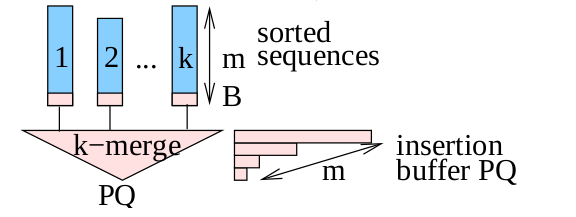
\includegraphics[width=0.8\textwidth]{external_pq.png}
\end{figure}



Internal Storage: ein insertion PQ-Puffer mit Größe $m$ (konstanter Anteil von $M$) und eine deletion PQ die effektiv ein k-merge implementiert. Die deletion PQ speichert jeweils das kleinste Element einer Sequenz, zusammen mit dem Sequenzindex. Zudem sind jeweils bis zu $B$ Sequenzen im internal Memory gespeichert, die verbleibenden Blöcke im external Memory.
 
Insertions werden nur bei Überlaufen in die Sequenzen geschrieben.
Deletions erfolgen aus der PQ mit dem kleineren Minimum.
Amortisiert $O(1/B)$ I/O-Zugriffe.

Die interne Analyse bezieht sich vor allem auf den Aufwand für das erneute Sortieren der bestehenden Strukturen und beläuft sich auf $O(log m)$ 

\section{Externe minimale Spannbäume}
Annahme: $M=\Omega(n)$ konstant viele Worte pro Knoten. Also Knoten im Speicher, Kanten draußen.

Sortiere Kanten nach aufsteigendem Gewicht. Initialisiere Treekomponenten als jeweils ihren eigenen Knoten. Füge dann iterativ die Kanten hinzu, die nicht innerhalb derselben Komponente liegen.
